
%%%%% Content %%%%%

In normal Logic we only differentiate if a statement is true or false. But if we want to model the real world, there are some statements which cannot clearly be decided as true or false, e.g. the car is comfortable or the car is old. This can be modelled by fuzzy sets.


%%% §1 %%%
\section{Fuzzy Sets}
In regular crisp set theory an element $x$ of a (crisp) set $\Omega$ either belongs to a (crisp) subset $A$ or not. In Fuzzy Logic we define a (membership) value $\ol A(x)\in[0,1]$ for an element $x\in\Omega$, which describes the membership of $x$ to a subset $A$. So in case of a crisp set $A$ we have $\ol A(x)=1$ if $x\in A$ and if $x\notin A$, then $\ol A(x)=0$.

\subsection{Knowledge Representation in a fuzzy set}
In normal speech the age of a person is not always described with the exact age, mostly some description as \emph{young}, \emph{old}, \emph{around 40} or \emph{between 30 and 40} is used. \\
This should be modelled by fuzzy set theory too, so a fuzzy set should not only model numerical variables, it should also be able to model linguistic variables like \emph{age}, \emph{speed} or \emph{temperature}, \qq{whose (linguistic) values are words or sentences in a natural or artificial language}\cite{IntrFuzzyControl}. \\
Therefore a fuzzy set can contain different types of elements:
\begin{itemize}
\item Real Numbers,
\item Fuzzy Numbers (e.g. \emph{approximately 4} or \emph{(approximately) between 3 and 4}; see \ref{sec:fuzzyNumbers}),
\item Linguistic values (e.g. \emph{large}, \emph{very large}, \emph{old}, \emph{young}, \emph{pretty} or \emph{nice}; see \ref{sec:linguicVar}).
\end{itemize}


\subsubsection{Linguistic Variables and Values} \label{sec:linguicVar}
As mentioned above, linguistic variables are described by linguistic values. But for the calculation with linguistic variables we need some numerical representation or information of the linguistic values.\\
Therefore a linguistic variable is associated with the following notion:
\[ \langle X,\mc LX, \mc X, M_X \rangle, \]
where:
\begin{itemize}
\item[$X$] is the \emph{symbolic name} of the linguistic variable (e.g. age, speed or temperature)
\item[$\mc LX$] is the \emph{set of linguistic values} (also \emph{term-set}, \emph{reference-set}), that $X$ can take (e.g. young, middle, old for age or (very) slow, normal, (very) fast for speed)
\item[$\mc X$] is the \emph{physical domain} (also \emph{universe of discourse}) over which the (linguistic) variable $X$ takes its quantitative (crisp) values (e.g. the interval $[0$ km/h, $400$ km/h $]$ for speed)
\item[$M_X$] is a \emph{semantic function} that refers to every element (linguistic value) $LX\in\mc LX$ a physical, so quantitive, meaning or interpretation. This meaning/interpretation is represented by a fuzzy set $\widehat{LX}$, that is defined over $\mc X$ (e.g. a car is fast if it drives (at least) approximately $100$ km/h, see \ref{sec:fuzzyNumbers} for a possible fuzzy number that models this). Ofttimes also the membership function $\mu_{LX}:=M_X(LX)$ is used.
\end{itemize}
As an example, we can define a fuzzy (sub-)set $\ol A$ of $\{ very\, small, small, medium, high, very\, high \}$ that models e.g. the height of trees:
\[ \ol A(small)=0.3,\quad \ol A(medium)=1.0, \quad \ol A(high)=0.7. \]
$\ol A$ is a \textbf{discrete fuzzy set} and is commonly written as
\[ \ol A = \left\{ \frac{0.3}{small}, \frac{1.0}{medium}, \frac{0.7}{high} \right\}. \]
For this example we then can define the linguistic variable $X=H:=$ \textit{height (of trees)}, term-set $\mc LH=\{ very\, small, small, medium, high, very\, high \}$, universe of discourse $\mc H=[0$ m, $60$ m$]$ and the semantic/membership function $M_H$, respectively $\mu_{LH}$, defined as following:
\begin{align*}
\mu_{small}(x) = M_H(small)(x) :=& \ \begin{cases}
		1, &x \leq 8 \\
		\frac{16-x}{8}, &8 < x < 16 \\
		0, &x \geq 16
	\end{cases} \\
	 \widehat{=}& \quad \qq{\text{height is less than $16$m.}} \\
\mu_{medium}(x) = M_H(medium)(x) :=& \ \begin{cases}
		0, &x \leq 8 \\
		\frac{x-8}{8}, & 8 < x < 16 \\
		1, &x = 16 \\
		\frac{24-x}{8}, &16 < x < 24 \\
		0, &x \geq 24
	\end{cases} \\
	\widehat{=}& \quad \qq{\text{height is about $16$m.}} \\
\mu_{high}(x) = M_H(high)(x) :=& \ \begin{cases}
		0, &x \leq 16 \\
		\frac{x-16}{8}, &16 < x < 24 \\
		1, &x \geq 24
	\end{cases} \\
	\widehat{=}& \quad \qq{\text{height is more than $16$m.}}
\end{align*}
$\mu_{small},\, \mu_{medium}$ and $\mu_{high}$ are socalled \emph{fuzzy numbers} (\ref{sec:fuzzyNumbers})  and can be illustrated as following:
\begin{figure}[H]
\centering
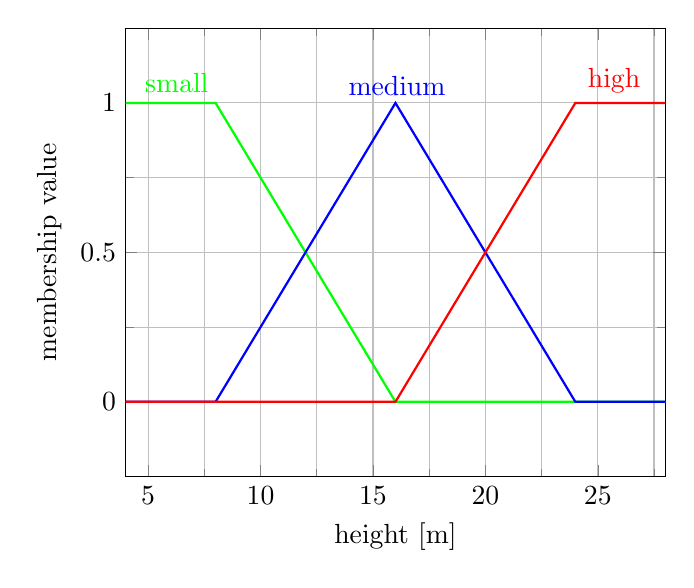
\begin{tikzpicture}
	\begin{axis}[grid=both,ymin=-0.25,ymax=1.25,xmin=4,xmax=28,
               minor tick num=1,
               %axis lines = middle,
               xlabel=\text{height [m]},ylabel=\text{membership value},
               %legend style={at={(axis cs:40,0.5)},anchor=east}
               ]
		% add line "small"\\
		%\addlegendentry{small}
		\addplot [mark=none,green,thick] coordinates { (4,1) (8,1) (16,0) (45,0) } node [pos=0.01,above right] {small};
		% add line "medium"
		%\addlegendentry{medium}
		\addplot [mark=none,blue,thick] coordinates { (4,0) (8,0) (16,1) (24,0) (45,0) } node [pos=0.295,above] {medium};
		% add line "high"
		%\addlegendentry{high}
		\addplot [mark=none,red,thick] coordinates { (4,0) (16,0) (24,1) (45,1) }node [pos=0.57,above left] {high};
  \end{axis}
\end{tikzpicture}
\end{figure} \FigureHSpace
Therefore the linguistic variable \textit{height} is in our case associated with this notion:
\[ \langle H, \mc LH, \mc H, M_H \rangle = \langle height, \{ very\, small, small, medium, high, very\, high \}, [0,60], M_H \rangle.\]

\subsection{Arithmetic of fuzzy sets} \label{sec:fuzzyArithm}
As in the regular sets theory we want to define the intersection $\ol A\cap\ol B$, the union $\ol A\cup\ol B$ and the complement $\ol A^c$ of $\ol A$:\\
The \emph{complement} is defined via the membership-function
\[ \ol A^c(x) = 1-\ol A(x). \]
The \emph{intersection} for fuzzy sets $\ol A,\ol B$ defined on the same support $X:=\SUPP(\ol A)=\SUPP(\ol B)$ can be defined by ($x\in X$)
\[ (\ol A\cap\ol B)(x) = T(\ol A(x),\ol B(x)), \]
for a so-called \emph{t-norm} $T$, that has the following specifications ($x\in X$):
\begin{enumerate}[1)]
\item $T(\ol A(x),1)=\ol A(x)$
\item $T(\ol A(x),\ol B(x))=T(\ol B(x),\ol A(x))$ (Symmetry)
\item if $\ol B_1(x)\leq \ol B_2(x)$, then $T(\ol A(x),\ol B_1(x))\leq T(\ol A(x),\ol B_2(x))$ (Monotony)
\item $T(\ol A(x),T(\ol B(x),\ol C(x)))=T(T(\ol A(x),\ol B(x)),\ol C(x))$ (Associative)
\end{enumerate}
Note that $T(1,1)=1, T(0,1)=T(1,0)=T(0,0)=0$, so if it is reduced to crisp sets we obtain exactly the intersection $A\cap B$ for crisp sets.\\
Similar as above, the \emph{union} for fuzzy sets $\ol A,\ol B$ defined on the same support $X:=\SUPP(\ol A)=\SUPP(\ol B)$ can be defined by ($x\in X$)
\[ (\ol A\cup\ol B)(x) = C(\ol A(x),\ol B(x)), \]
for a so-called \emph{t-conorm} $C$, that has the following specifications:
($x\in X$)
\begin{enumerate}[1)]
\item $C(\ol A(x),0)=\ol A(x)$
\item $C(\ol A(x),\ol B(x))=C(\ol B(x),\ol A(x))$ (Symmetry)
\item if $\ol B_1(x)\leq \ol B_2(x)$, then $C(\ol A(x),\ol B_1(x))\leq C(\ol A(x),\ol B_2(x))$ (Montony)
\item $C(\ol A(x),C(\ol B(x),\ol C(x)))=C(C(\ol A(x),\ol B(x)),\ol C(x))$ (Associative)
\end{enumerate}
Note that $C(1,1)=C(0,1)=C(1,0)=1, C(0,0)=0$, so if it is reduced to crisp sets we obtain exactly the union $A\cup B$ for crisp sets.


\subsubsection*{Cylindrical Extension} \label{sec:cylindExt}
If the support of $\ol A$ and $\ol B$ is not the same (e.g. $\ol A$ and $\ol B$ are describing different aspects like age and speed of cars), the \emph{cylindrical extension} is a possibility to obtain the intersection/union:\\
The idea of the cylindrial extension is to define a fuzzy relation between the fuzzy sets $\ol A$ and $\ol B$. Therefore we define extensions $\ol A^*$ and $\ol B^*$ that are defined on $\SUPP(\ol A)\times\SUPP(\ol B)$:
\[ A^*(x_1,x_2) = A(x_1), \quad \forall x_2\in\SUPP(\ol B),x_1\in\SUPP(\ol A) \]
and
\[ B^*(x_1,x_2) = B(x_2), \quad \forall x_1\in\SUPP(\ol A),x_2\in\SUPP(\ol B) \]
Now we can calculate the resulting $\ol C_{inter} = \ol A^*\cap\ol B^*$ and $\ol C_{union} = \ol A^*\cup\ol B^*$ on $\SUPP(\ol A)\times\SUPP(\ol B)$ with an intersection- and union-operator.

\vspace*{0.75cm} \hspace*{-1.5em}
With these definitions of a t-norm and t-conorm we can obtain (at least most of) the rules of regular sets theory for fuzzy sets (without proof):
\begin{itemize}
\item Idempotency,
\item Commutativity (respect to $\cup, \cap$),
\item Associativity (respect to $\cup, \cap$),
\item Absorption,
\item Distributivity,
\item Identity,
\item Law of Contradiction,
\item Law of Excluded Middle,
\item Involution,
\item De Morgan laws.
\end{itemize}
Examples of t-norms are (on a set $X=X_1\times X_2$, where $A$ is defined on $X_1$, $B$ on $X_2$ and $(x,y)\in X_1\times X_2$):
\begin{itemize}
\item Standard intersection:
	\[ T_m(\ol A(x),\ol B(y)) = \min(\ol A(x),\ol B(y)) \]
\item Bounded sum:
	\[ T_b(\ol A(x),\ol B(y)) = \max(0, \ol A(x)+\ol B(y)-1) \]
\item Algebraic product:
	\[ T_p(\ol A(x),\ol B(y)) = \ol A(x)\cdot\ol B(y) \]
\item Drastic intersection:
	\[ T^*(\ol A(x),\ol B(y)) = \begin{cases}
	\ol A(x), &\text{if } \ol B(y)=1,\\
	\ol B(y), &\text{if } \ol A(x)=1,\\
	0, \text{otherwise}
	\end{cases} \]
\end{itemize}
The advantage of $T_m$ is the fast and easy calculation, but there's no difference in the intersection if $\ol A_1(x)>\ol A_2(x)>\ol B(x)$, so we lose information about $\ol A$ (resp. $\ol A_1,\ol A_2$), since only the value $\ol B(x)$ will be used. Therefore $T_p$ is sometimes better since the information from both fuzzy sets will be used. But the choice of the intersection-operator is dependent on the application.\\
It states (for better readability without arguments):
	\[ T^* \leq T_b \leq T_p \leq T_m,\text{ in fact: } T^* \leq T \leq T_m,\quad\forall\, t\text{-norms } T. \]
Examples of t-conorms are (on a set $X=X_1\times X_2$, where $A$ is defined on $X_1$, $B$ on $X_2$ and  $(x,y)\in X_1\times X_2$):
\begin{itemize}
\item Standard union:
	\[ C_m(\ol A(x),\ol B(y)) = \max(\ol A(x),\ol B(y)) \]
\item Bounded sum:
	\[ C_b(\ol A(x),\ol B(y)) = \min(1, \ol A(x)+\ol B(y)) \]
\item Algebraic sum:
	\[ C_p(\ol A(x),\ol B(y)) = \ol A(x)+\ol B(y) - \ol A(x)\cdot\ol B(y) \]
\item Drastic union:
	\[ C^*(\ol A(x),\ol B(y)) = \begin{cases}
	\ol A(x), &\text{if } \ol B(y)=0,\\
	\ol B(y), &\text{if } \ol A(x)=0,\\
	1, \text{otherwise}
	\end{cases} \]
\end{itemize}
As with t-norms the choice of the union-operator is dependent on the application.\\
It states (for better readability without arguments):
\[ C_m \leq C_p \leq C_b \leq C^* \text{ in fact: } C_m \leq C \leq C^*,\quad\forall\, t\text{-conorms } C. \]

$T$ and $C$ are called \emph{dual} $:\Leftrightarrow$ $\begin{cases}
T(\ol A(x),\ol B(y)) = 1 - C(1-\ol A(x), 1-\ol B(y)) \\
C(\ol A(x),\ol B(y)) = 1 - T(1-\ol A(x), 1-\ol B(y))
\end{cases}$.


\subsection{Logical Rules} \label{sec:logicRules}
In this part we want to calculate logical connections between fuzzy statements like
\begin{center}
IF ( (a car is older than 30 years) AND (a car is fast) ) THEN (a car is expensive).
\end{center}
or
\begin{center}
IF ( (a car is older than 30 years) OR (a car is fast) ) THEN (a car is expensive).
\end{center}
In part \ref{sec:fuzzyArithm} we learned amongst building the complement how to intersect and unite fuzzy sets. Therefore by identifying the complement with the negation $\neg$, union with OR, intersection with AND, $\emptyset$ with $0$ and the \emph{support $X$} with $1$ we get a connection between calculations of fuzzy sets and fuzzy logic. For a complete logical model we also need the implication, which we will derive in this chapter. To clarify we show the connection between fuzzy sets and fuzzy logic with the examplary statements above: \\
If we have the fuzzy set $\ol A_1$ of cars older than 30 years and the fuzzy set $\ol A_2$ of fast cars and want to calculate the set $\ol B$ of fast cars that are older than 30 years, we obtain this via
\[ \ol B = \ol A_1\cap\ol A_2. \]
Respectively, if we want to compute the (fuzzy) set $\ol C$ of fast cars or cars older than 30 years, we get
\[ \ol C = \ol A_1\cup\ol A_2. \]
The resulting set is hereby dependent on the choice of the intersection- resp. the union-operator (compare \ref{sec:fuzzyArithm}).\\
For the implication we can make use of the following fact (let $p,q$ be statements):
\[ \text{IF } p \text{ THEN } q \Leftrightarrow \neg p \text{ OR } q \]
Then we can calculate the \emph{fuzzy implication} $\ol A\rightarrow\ol B$ with support $X_1\times X_2$ as following:
\[ (\ol A\rightarrow\ol B)(x,y) = C(1-\ol A(x), \ol B(y)), \quad (x,y)\in X_1\times X_2 \]
with a t-norm $C$, e.g. $C_m$:
\[ (\ol A\rightarrow\ol B)(x,y) = max(1-\ol A(x), \ol B(y)), \]
Another common implication operator is the \emph{Mamdani implication operator}:
\[ (\ol A\rightarrow\ol B)(x,y) = \min(\ol A(x), \ol B(y)).\]
It is based on the assumption that the truth-value of the conclusion $\ol B(y)$ cannot be higher than the truth-value of the premise $\ol A(x)$.


\subsection{Fuzzy Numbers} \label{sec:fuzzyNumbers}
Fuzzy numbers are special fuzzy sets. They express e.g. approximately a (crisp) number, an interval of the real numbers or just values \qq{(much) bigger/smaller than} a real value (compare \ref{sec:linguicVar}). \\
From \cite{IntrFuzzyLogic} we obtain the following definition of fuzzy numbers:

A fuzzy number $\ol N$ is a fuzzy subset of $\R$ with following restrictions:
\begin{enumerate}[(i)]
\item The core of $\ol N$ is non-empty ($\Leftrightarrow \exists x: \ol N(x)=1$).
\item $\alpha$-Cuts of $\ol N$ (explained in the following section) are all closed and bounded intervals.
\item The support $\{ x | \ol N(x)>0 \}$ of $\ol N$ is bounded.
\end{enumerate}
Since the core of $\ol N$ should be non-empty, $\ol N$ must be a normal fuzzy set, that means there is at least one $x$, such that $\ol N(x)=1$.


%\cite{SimulatingFuzzySystems}
\subsubsection*{Special Case}
A special case of fuzzy numbers are \emph{triangular} or \emph{triangular shaped} fuzzy numbers. They are defined by three numbers $a<b<c$, where the positive values of the fuzzy number are in the interval $(a,c)$ and the maximum value $1$ is at point $b$.\\
A \emph{triangular} fuzzy number has linear connection lines between $\ol N(a)$ to $\ol N(b)(=1)$ and from $\ol N(b)$ to $\ol N(c)$. For such a fuzzy number we write $\ol N=(a/b/c)$.\\
A \emph{triangular shaped} fuzzy number has to be continuous (or rather the graph of $\ol N$), monotonically increasing on $[a,b]$ and monotonically decreasing on $[b,c]$. We denote such a fuzzy number as $\ol N\approx (a/b/c)$.

Besides the triangular (shaped) fuzzy numbers, there is another big set of common fuzzy numbers: \emph{trapezoidal (shaped)}. They are described via $\ol T=(a/b,c/d)$ and it states: $\ol T([b,c])=\{1\}$. As the triangular (shaped) fuzzy numbers they have the same monotoneous requirements.

%\cite{IntrFuzzyLogic}
As an example, a triangular shaped fuzzy number $(1/2/3)$ is expressing \emph{approximately $2$}, a fuzzy interval $(1.5/3,5/6.5)$ is expressing a number \emph{approximately between $3$ and $5$}:
\begin{figure}[H]
\centering
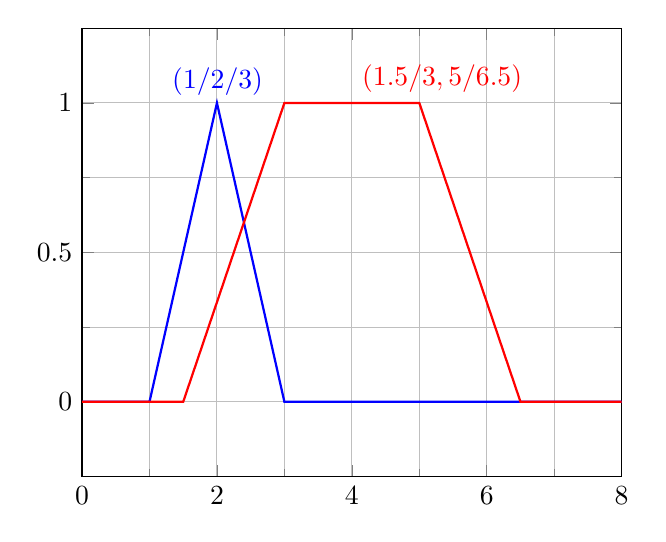
\begin{tikzpicture}
	\begin{axis}[grid=both,ymin=-0.25,ymax=1.25,xmin=0,xmax=8,
               minor tick num=1,
               %axis lines = middle,
               %xlabel=\text{height [m]},
               %ylabel=\text{},
               %legend style={at={(axis cs:40,0.5)},anchor=east}
               ]
		% add line
		%\addlegendentry{small}
		\addplot [mark=none,blue,thick] coordinates { (0,0) (1,0) (2,1) (3,0) (8,0) } node [pos=0.275, above] {$(1/2/3)$};
		% add line
		%\addlegendentry{medium}
		\addplot [mark=none,red,thick] coordinates { (0,0) (1.5,0) (3,1) (5,1) (6.5,0) (8,0) } node [pos=0.5, above right] {$(1.5/3,5/6.5)$};
  \end{axis}
\end{tikzpicture}
\end{figure} \FigureHSpace

\subsubsection{$\alpha$-Cuts} \label{sec:alphaCuts}
An $\alpha$-Cut $\ol A[\alpha]$ of a fuzzy number $\ol A$ with $\ol A>0$ on $[a,c]$ is defined by:
\[ \ol A[\alpha] := \{ x\in\Omega | \ol A(x)\geq\alpha \}\subset[a,c] \quad \forall\alpha\in(0,1] \]
\[ \ol A[0] := [a,c]. \]
$\ol A[0]$ is called the \emph{support or base of $\ol A$}.\\
$\ol A[1]$ is called the \emph{core of $\ol A$}.\\
So for a triangular or triangular shaped fuzzy number $\ol N=(a/b/c)$ we obtain $\ol N[1]=\{b\}$ and %\cite{SimulatingFuzzySystems}
for a trapezoidal (shaped) fuzzy number $\ol N=(a/b,c/d)$ we get $\ol N[1]=[b,c]$.

We also know (without proof) that an $\alpha$-Cut $\ol Q[\alpha]$ for a fuzzy number $\ol Q$
is a closed and bounded interval ($0\leq\alpha\leq 1$):
\[ \ol Q[\alpha]=[q_1(\alpha), q_2(\alpha)], \]
where $q_1(\alpha)$ is an increasing, $q_2(\alpha)$ a decreasing function of $\alpha$ and $q_1(1)=q_2(1)$.


\subsubsection{Fuzzy Arithmetic}
There are two (\todo{why?}{equivalent}; without proof) ways of adding, subtracting, multiplying and dividing two fuzzy numbers:\\
\begin{itemize}
\item \todo{explain better: Norms $T$...}{Extension principle}: For $\ol C:=\ol A \ast \ol B,\quad \ast\in\{+,-,\cdot,/ \}$ we define:
	\[ \ol C:=\sup_{x,y} \{ \min(\ol A(x),\ol B(y))\, |\, x\ast y=z \} \]
	%Here the \emph{standard intersection $t$-norm} $T_m(a,b)=\min(a,b)$ was used for the extension principle (extension of the universe of discours). (compare \ref{sec:fuzzyArithm})
\item \todo{explain more?}{Interval Arithmetic/$\alpha$-Cuts}: For $\ol C:=\ol A \ast \ol B \quad\ast\in\{+,-,\cdot,/ \}$ we define:
	\[ \ol C[\alpha]:=\ol A[\alpha] \ast \ol B[\alpha] \]
\end{itemize}


%Let $\ol A,\ol B$ bew two fuzzy subsets of a set $\Omega$. Then we define:
%\begin{align*}
%\ol A\leq\ol B \quad &:\Leftrightarrow \ol A(x)\leq\ol B(x), \forall x\in\Omega\quad (\ol A \text{ is a fuzzy subset of } \ol B) \\
%\ol A<\ol B \quad &:\Leftrightarrow \ol A(x)<\ol B(x),\quad \forall x\in\Omega \quad(??\text{ or is it }\forall x\in support(\ol A)\cap support(\ol B) ??)
%\end{align*}


\subsubsection{Ordering fuzzy numbers}
Since we have a total ordering $(<,\leq,=)$ on the real numbers, we would like to have such a total ordering on the fuzzy numbers (as an extension of the real numbers) too, or at least a partial ordering (meaning: $\ol A\geq\ol B$ or $\ol A\leq\ol B$ not for all fuzzy numbers $\ol A,\ol B$).
For $\delta\in\R$ and a fuzzy number $\ol N=(a/b/c)$ or $\ol N\approx(a/b/c)$ we write $\ol N\geq(>)\,\delta$ if $a\geq(>)\,\delta$ and $\ol N\leq(<)\,\delta$ if $c\leq(<)\,\delta$.

There are a few definitions of $(<,\leq,\approx/=)$ between fuzzy numbers, but not all fulfilling the axioms of a total ordering (partial ordering: without point 4):
\begin{enumerate}[1.]
\item reflexive
\item transitive
\item $\ol M\leq\ol N$ and $\ol M\leq\ol N\, \Rightarrow\, \ol M\approx\ol N$
\item $\ol M\leq\ol N$ or $\ol M\leq\ol N\quad \forall \ol M,\ol N$
\end{enumerate}

In this section we want to present one possible definition for the meaning of the symbols $\leq,<$ and $\approx$ for fuzzy numbers. In \cite{SimulatingFuzzySystems} the following definition is introduced:
\[ v(\ol M\leq\ol N)=\max\{ \min(\ol M(x), \ol N(y))\, |\, x\leq y \} \]
and
\begin{align*}
\ol N < \ol M &:\Leftrightarrow v(\ol N \leq \ol M)=1 \text{ and } v(\ol M \leq \ol N)<\eta \in (0,1] \text{ fixed} \\
\ol N \approx \ol M &:\Leftrightarrow \text{neither } \ol N<\ol M \text{ nor } \ol M<\ol N \text{ is correct} \\
\ol N \leq \ol M &:\Leftrightarrow \ol N < \ol M \text{ or } \ol N\approx\ol M.
\end{align*}
Because of being the highest value  two fuzzy numbers $M$ and $N$ have in common (in respect to $x\leq y, x\in$ support $M$, $y\in$ support $N$), $\eta$ is a regulating value for $M$ and $N$ being equal or $M$ smaller (bigger) than $N$.
\begin{align*}
v(\ol N \leq \ol M) = 1 &\Leftrightarrow \max\{ \min(\ol N(x), \ol M(y))\, |\, x\leq y \} = 1 \\
&\Leftrightarrow \exists x\in\SUPP(\ol N),y\in\SUPP(\ol M) \text{ with } x\leq y: \min(\ol N(x), \ol M(y)) = 1 \\
&\Leftrightarrow \exists x\in\SUPP(\ol M),N\in\SUPP(\ol M) \text{ with } x\leq y: \ol N(x) = 1 = \ol M(y) \\
&\Leftrightarrow \text{The left border of the core of $\ol N$ lies left of one element of the core of $\ol M$}. \\
v(\ol M \leq \ol N) < \eta &\Leftrightarrow \max\{ \min(\ol M(x), \ol N(y))\, |\, x\leq y \} < \eta \\
&\Leftrightarrow \exists x\in\SUPP(\ol M),y\in\SUPP(\ol N) \text{ with } x\leq y: \min(\ol M(x), \ol N(y)) < \eta \\
&\Leftrightarrow \exists x\in\SUPP(\ol M),y\in\SUPP(\ol N) \text{ with } x\leq y: \ol M(x), \ol N(y) \geq \eta \\
&\Leftrightarrow \text{$\eta$ is the highest number $\ol M$ and $\ol N$ have in common in respect to $x\leq y$}.
\end{align*}
With this ordering we obtain some clustering depending on $\approx$ and $\leq/<$.\\
With such an relation/ordering on the fuzzy numbers we can calculate the min. and max. value of a set of fuzzy numbers.


\subsection{Fuzzy Functions}
As for functions $h\colon [a,b]\rightarrow\R$ in the real numbers we can also obtain a (fuzzy) function $H(\ol X)=\ol Z$ on fuzzy numbers. This can be done by the \emph{extension principle} (\ref{sec:extPrincFunc}) or \emph{interval arithmetic/$\alpha$-Cuts} (\ref{sec:intArithmFunc}).

\subsubsection{Extension Principle} \label{sec:extPrincFunc}
\todo[inline,color=green]{explain more/better}
We extend a real number function $h\colon [a,b]\rightarrow\R$ to $\ol Z=H(\ol X)$ by the following definition:
\[ \ol Z(z):=\sup_x\{ \ol X(x) | h(x)=z,\, a \leq x \leq b \}. \]
For the $\alpha$-Cuts $\ol Z[\alpha]=[z_1(\alpha), z_2(\alpha)]$ of a fuzzy number $\ol Z$ \todo{why exactly?}{it lasts}, if $h$ is continuous (without proof):
\begin{align*}
z_1(\alpha) &= \min\{ h(x) | x\in\ol X[\alpha] \} \\
z_2(\alpha) &= \max\{ h(x) | x\in\ol X[\alpha] \}
\end{align*}

\subsubsection{Interval Arithmetic/$\alpha$-Cuts} \label{sec:intArithmFunc}
\todo[inline,color=green]{explain more/better}
To extend a real number function $h$ (see above) with interval arithmetic and $\alpha$-Cuts, we calculate $H(\ol X[\alpha])=\ol Z[\alpha]$. If there are other fixed fuzzy numbers used in $H(\ol X)$, then we use their $\alpha$-Cuts too for the computation.

%\subsubsection{Differences}
%We denote $\ol Z^*=H(\ol X)$ for the extension of $h\colon [a,b]\rightarrow\R$ with the extension principle and $\ol Z=H(\ol X)$ for the calculation with interval arithmetic and $\alpha$-Cuts.\\
%\todo{whereever??}{We know} that $\ol Z^*\leq \ol Z$ \qq{for usual functions in science and engineering}.
%
%\subsubsection*{Example}
%We have $\ol Z=(1-\ol X)\ol X$ with $\ol X$ a triangular fuzzy number in $[0,1]$. For $\ol X[\alpha]=[x_1(\alpha), x_2(\alpha)]$ we get (interval arithmetic !):
%\[ \ol Z[\alpha] = (1-\ol X[\alpha])\ol X[\alpha]=[z_1(\alpha), z_2(\alpha)] \]
%And since $1-\ol X(\alpha)\leq 0,\ol X(\alpha)\geq 0$, we know for interval aritmetic ($b_1<0, a_2\geq0$):
%\[ [a_1,a_2]\cdot[b_1,b_2] = [a_1b_2,a_2b_1] \]
%This leads to:
%\begin{align*}
%z_1(\alpha) &= (1-x_1(\alpha))x_2(\alpha)\\
%z_2(\alpha) &= (1-x_2(\alpha))x_1(\alpha)
%\end{align*}
%From the extension principle we get:
%\[ \ol Z^*(z) = \sup_x\{ \ol X(x) | (1-x)x=z,\, 0 \leq x \leq 1 \} \]
%We write $\ol Z^*[\alpha]=[z_1^*(\alpha), z_2^*(\alpha)]$ and since $h$ is continuous we obtain:
%\begin{align*}
%z_1^*(\alpha) &= \min\{ (1-x)x | x\in\ol X[\alpha] \} \\
%z_2^*(\alpha) &= \max\{ (1-x)x | x\in\ol X[\alpha] \}
%\end{align*}
%That is not the same (see the exact counter example in the book!) as the above $z_1(\alpha),z_2(\alpha)$.\\
%However, \todo{where? Proof?}{we know} that the inverval arithmetic- and the extension principle will produe the same result if the independent fuzzy number variables $\ol X,\ldots$ appear only once in the expression of the function!


%%% §2 %%%
\newpage
\section{Fuzzy Models}
The basic principle of a fuzzy model is illustrated and described in this chapter.

\begin{figure}[H]
\centering

% Define block styles
\tikzstyle{plain} = [draw=none, text width=3em, text centered]
\tikzstyle{block} = [rectangle, draw, text width=8em, text centered]
\tikzstyle{arrow} = [draw, -latex']

\resizebox{\linewidth}{!}{
	\begin{tikzpicture}[every node/.style={font=\footnotesize}, node distance=5cm, auto, >=latex']
		% Place nodes
		\node [plain] (input) {crisp input values};
		\node [block, right of=input, node distance=3.5cm] (fuzzi) {FUZZIFICATION\\- calculating membership values};
		\node [block, right of=fuzzi, node distance=5.5cm] (inter) {INTERFERENCE\\- rules\\- aggregation\\- interference};
		\node [block, right of=inter] (defuz) {DEFUZZIFICATION\\- calculating crisp output values};
		\node [plain, right of=defuz, node distance=3.5cm] (output) {crisp output values};

		% Draw edges
		\path[->] ([yshift=0.5cm]input.east) edge node[above] {$x_1^{\ast}$} node [below] {$\vdots$} ([yshift=0.5cm]fuzzi.west);
   	\path[->] ([yshift=-0.5cm]input.east) edge node[below] {$x_n^{\ast}$} ([yshift=-0.5cm]fuzzi.west);
		\path[->] (fuzzi) edge node[above] {member-} node[below] {ship values} (inter);
   	\path[->] ([yshift=0.5cm]inter.east) edge node[above] {$\mu(y_1)$} node [below] {$\vdots$} ([yshift=0.5cm]defuz.west);
   	\path[->] ([yshift=-0.5cm]inter.east) edge node[below] {$\mu(y_n)$} ([yshift=-0.5cm]defuz.west);
   	\path[->] ([yshift=0.5cm]defuz.east) edge node[above] {$y_1^{\ast}$} node [below] {$\vdots$} ([yshift=0.5cm]output.west);
   	\path[->] ([yshift=-0.5cm]defuz.east) edge node[below] {$y_n^{\ast}$} ([yshift=-0.5cm]output.west);
	\end{tikzpicture}
}
\end{figure} \FigureHSpace
In a fuzzy model we get $n$ crisp input and $m$ crisp output values. Therefore, to work with fuzzy logic/variables, we first have to calculate the membership values in particular fuzzy sets (called \emph{Fuzzification}).\\
The next block, which gets the membership values as an input, is called \emph{Interference}. The rules of the fuzzy system will be applied here following this mechanism:
\begin{itemize}
\item rule base: consists of logicaI rules determining causal relationships
existing in the system between fuzzy sets of its inputs and outputs, e.g. one examplary rule for a $2$-input, $1$-ouput model:
	\begin{center} IF $(x_1=A_1)$ AND $(x_2=B_1)$ THEN $(y=C_1)$, \end{center}
	where $x_1,x_2$ and $y$ are the fuzzy input values and $A_1,B_1$ and $C$ are the fuzzy reference values.
\item interference mechanism:
	\begin{itemize}
	\item calculating the results of the rules: Usage of the fuzzy logic (see \ref{sec:logicRules}) and (mostly) via \emph{Generalized Modus Ponens}, which states, that if we have the following rule:
		\begin{center} IF $(x=small)$ THEN $(y=big)$ \end{center}
	and $x^*$ is \textit{very} small, then it follows that $y^*$ is \textit{very} big.
	\item \emph{aggregation} of the results of the rules and calculating the resulting membership-function. As an illustration: If we have two rules
		\begin{center} (R1) $\qquad$ IF $(x_1=A_1)$ THEN $(y=C_1)$ \end{center}
		\begin{center} (R2) $\qquad$ IF $(x_1=A_2)$ THEN $(y=C_2)$, \end{center}
	then we get a membership value of $y$ for the fuzzy set $C_1$ and one for $C_2$.
	\end{itemize}
\end{itemize}
The last block \emph{Defuzzification} gets the calculated membership function values and calculates crisp, numeric output values $y_1^{\ast},\hdots,y_m^{\ast}$, being an effect of the numerical input values $x_1^{\ast},\hdots,x_n^{\ast}$. This operation is accomplished by a defuzzification mechanism determining the calculation method.


\subsection*{Example}
As an illustration we consider a 2-input, 1-output model. We want to calculate $y=x_1+x_2$, where $x_1$ and $x_2$ are input values in the universe of discourse $X=[0,10]$ and $y$ an output value in $Y=[0,20]$. In our fuzzy model we use the input fuzzy numbers \qq{small}, represented by $S_X=(0/0/10)$ and \qq{large}, represented by $L_X=(0/10/10)$. For the output we use crisp values \qq{small} ($S_Y=(0/0/0)$), \qq{medium} ($M_Y=(10/10/10)$) and \qq{large} ($L_Y=(20/20/20)$).\\
The next step in setting up our fuzzy model is to define the rules to obtain our rule base:
\begin{align*}
&\text{(R1)} & x_1=small &\text{ AND } x_2=small & &\text{THEN } y=small \\
&\text{(R2)} & (x_1=small \text{ AND } x_2=large) &\text{ OR } (x_1=large \text{ AND } x_2=small) & &\text{THEN } y=medium \\
&\text{(R3)} & x_1=large &\text{ AND } x_2=large & &\text{THEN } y=large.
\end{align*}
Written with fuzzy numbers we get:
\begin{align*}
&\text{(R1)} & x_1=S_X &\text{ AND } x_2=S_X & &\text{THEN } y=S_Y \\
&\text{(R2)} & (x_1=S_X \text{ AND } x_2=L_X) &\text{ OR } (x_1=L_X \text{ AND } x_2=S_X) & &\text{THEN } y=M_Y \\
&\text{(R3)} & x_1=L_X &\text{ AND } x_2=L_X & &\text{THEN } y=L_Y.
\end{align*}
For example, if we have two input values $x_1^*=2.5$ and $x_2^*=7.5$, we calculate their membership values of the fuzzy sets $S_X$ and $L_X$. These memberships values describe now, how big (respectively small) the crisp input values are (or rather to which amount they are a high (low) number).

\subsubsection*{Fuzzification}
Calculating the membership values for $x_1$ and $x_2$:
\begin{align*}
\mu_{S_X}(x_1) &= 0.75 & \\
\mu_{L_X}(x_1) &= 0.25 & \\
\mu_{S_X}(x_2) &= 0.25 & \\
\mu_{L_X}(x_2) &= 0.75. &
\end{align*}

\subsubsection*{Interference}
Calculating the results of the rules (\textit{AND} is modelled with the \qq{min-}, \textit{OR} with the \qq{max-Operator} and the \textit{implication} is just the identity):
\begin{enumerate}
\item[(R1)] $x_1=S_X \text{ AND } x_2=S_X \text{ THEN } y=S_Y$:\\
	\[ \mu_{(R1)}(y) = \mu_{S_Y}(y) = \ID\left( \min(\mu_{S_X}(x_1), \mu_{S_X}(x_2) ) \right) = \min(0.75, 0.25) = 0.25 \]
\item[(R2)] $(x_1=S_X \text{ AND } x_2=L_X) \text{ OR } (x_1=L_X \text{ AND } x_2=S_X) \text{ THEN } y=M_Y$:
	\begin{align*}
		\mu_{(R2)}(y) &= \mu_{M_Y}(y) = \ID\left(\, \max\left(\, \min(\mu_{S_X}(x_1), \mu_{L_X}(x_2) ), \min(\mu_{L_X}(x_1), \mu_{S_X}(x_2) ) \,\right) \,\right) \\
		&= \max\left( \min(0.75, 0.75), \min(0.25,0.25) \right) = 0.75
	\end{align*}
\item[(R3)] $x_1=L_X \text{ AND } x_2=L_X \text{ THEN } y=L_Y$:\\
	\[ \mu_{(R3)}(y) = \mu_{L_Y}(y) = \ID\left( \min(\mu_{L_X}(x_1), \mu_{L_X}(x_2) ) \right) = \min(0.25, 0.75) = 0.25 \]
\end{enumerate}

\subsubsection*{Aggregation}
In this example we chose the \qq{max}-mechanism for the aggregation of the resulting membership-values for $y$:
\[ \mu(y)= \max\left( \mu_{(R1)}(y), \mu_{(R2)}(y), \mu_{(R3)}(y) \right) = \max(0.25, 0.75, 0.25) = 0.75 = \mu_{M_Y}(y) \]

\subsubsection*{Defuzzification}
Since we have only crisp values as possible output values for $y$, there is no defuzzification mechanism needed and we get (since the aggregation mechanism tells us that we should look up the value in the fuzzy number \textit{medium}):
\[ y^{\ast} = 10. \]

Other examples have been done with the Matlab Toolbox \emph{Fuzzy Logic Design}.


%%%%% Content - END %%%%%

